\subsection{Mission overview}

The mission will consist of designing and building the rocket, the launch taking place in Bucharest, in which the rocket will be deployed, reaching, at the end of the ascent, a height of approximately 256m. During both the ascent and the descent, the sensors present in the rocket will measure the altitude, pressure, temperature, and acceleration, and through the GPS sensor, the information will be sent back and analysed. 

\subsection{Mechanical / structural design}

In this section, we will provide a detailed description of the rocket model’s mechanical design and the materials used for its structure, as well as the reasoning behind these choices. It also identifies the major components of the Payload, including the main board, sensors, transmitter, and battery, which will be detailed further in section 2.3. That subchapter will likewise include a preliminary drawing of how the Payload structure will look, where the major components will be placed, a list of sensors used, an explanation of the purposes of each component, and how they interact to accomplish our mission’s objectives.

\subsubsection{Mechanical Design}

The Rocket model structure is made of PLA and Acrylic, which provide strength and durability while keeping the overall weight of the Rocket model low. The structure has been designed to withstand the stress of launch and landing and includes a removable top for easy access to the interior components. The four fin sets are made out of balsa wood, for its lightweight, but structurally durable properties. The internal elements that need to withstand a greater force, such as the engine block, will be made of PLA, while the rest will be made of cardboard, for it is cheap and light. The components are mounted to the structure using screws and standoffs to provide a secure and stable platform for the electronic components, as well as relying on a tight and snug placement and bonding glues.

\subsubsection{Components}

The major components of the Payload include the main board, sensors, transmitter, and battery. The main board houses the microcontroller and provides the interface between the sensors and the transmitter. The sensors include a temperature sensor, a pressure sensor, and an altitude sensor. The transmitter is used to send data back to the ground station. The battery provides power to the Payload during the flight.

\begin{itemize}
    \item Nose Cone - with the shape of a tangent ogive
    \item Payload module - further described in chapter 2.3.
    \item Extra weight 10g
    \item Body tube - cylindrical
    \item Shock-Cord
    \item Parachute
    \item Bulkhead
    \item Fin sets - 4, of elliptical shape
    \item Engine block
    \item Centering rings
    \item Inner tube
    \item Launch lugs
    \item Motor
\end{itemize}

\subsubsection{Placement}

The Payload with the battery is placed inside the nose cone, with the sensors and transmitter located in its structure. The radio antenna will be placed in a way that allows it to communicate with the ground station, not being obscured by any other components after the release. The motor is placed in the lower part of the body tube, fixed by the inner tube and the centering rings. The engine block keeps the motor in place, being on top of it, and the bulkhead is placed over it, protecting the recovery system. On the side of the body tube we can find the launch lugs. The shoulder connects the body tube and the cone, the latter housing the Payload and its parachute, and the former containing the parachute and shock cord.

\subsubsection{Explanation}

The nose cone has the shape of a tangent ogive in order to be as aerodynamic as possible, thereby reducing air resistance. To ensure the stability of our rocket model, we might opt to add an extra weight in the cone, if the payload module doesn’t turn out to be heavy enough. The body tube will be made out of cardboard because we want to use a lightweight material that can also withstand the stress of launch and flight with high durability. The parachutes will be made out of Polyethylene, given that it is very thin, but resistant to shock and high forces, while the lines will be from braided nylon, and it will be tethered to the rocket model via an elastic shock cord. The bulkhead and engine block will be made of PLA, given that they need to withstand high shock forces. The inner tube will be from PLA, covering the motor, whereas the centering rings and launch lugs will be resistant enough to be made from cardboard, given its structural properties.

\subsection{Electrical design}

In this chapter we will present the exact details about the electrical design of the payload, including all the necessary components (controller and sensors) and how they will be connected. The power consumption of all the equipment will also be calculated, so that the perfect battery can be chosen. 

\subsection{Electrical interface}

The electrical interface has two main objectives: data collection and data transmission. The microcontroller used is an Arduino UNO R3, chosen for its convenient size and connectivity options. There is also an APC220 radio transmitter connected to the main board. All of this is powered by a 9V battery. There are 4 sensors connected to it:

\begin{itemize}
    \item MPU6050 (acceleration, orientation)
    \item NEO-6M (GPS)
    \item LM35DZ (temperature)
    \item BMP085 (atmospheric pressure)
\end{itemize}

Additionally, there is also an APC220 radio transmitter connected to the main board. All of this is powered by a 9V battery. Below is a scheme describing how all of these components come together:

\begin{figure}[H]
\centering
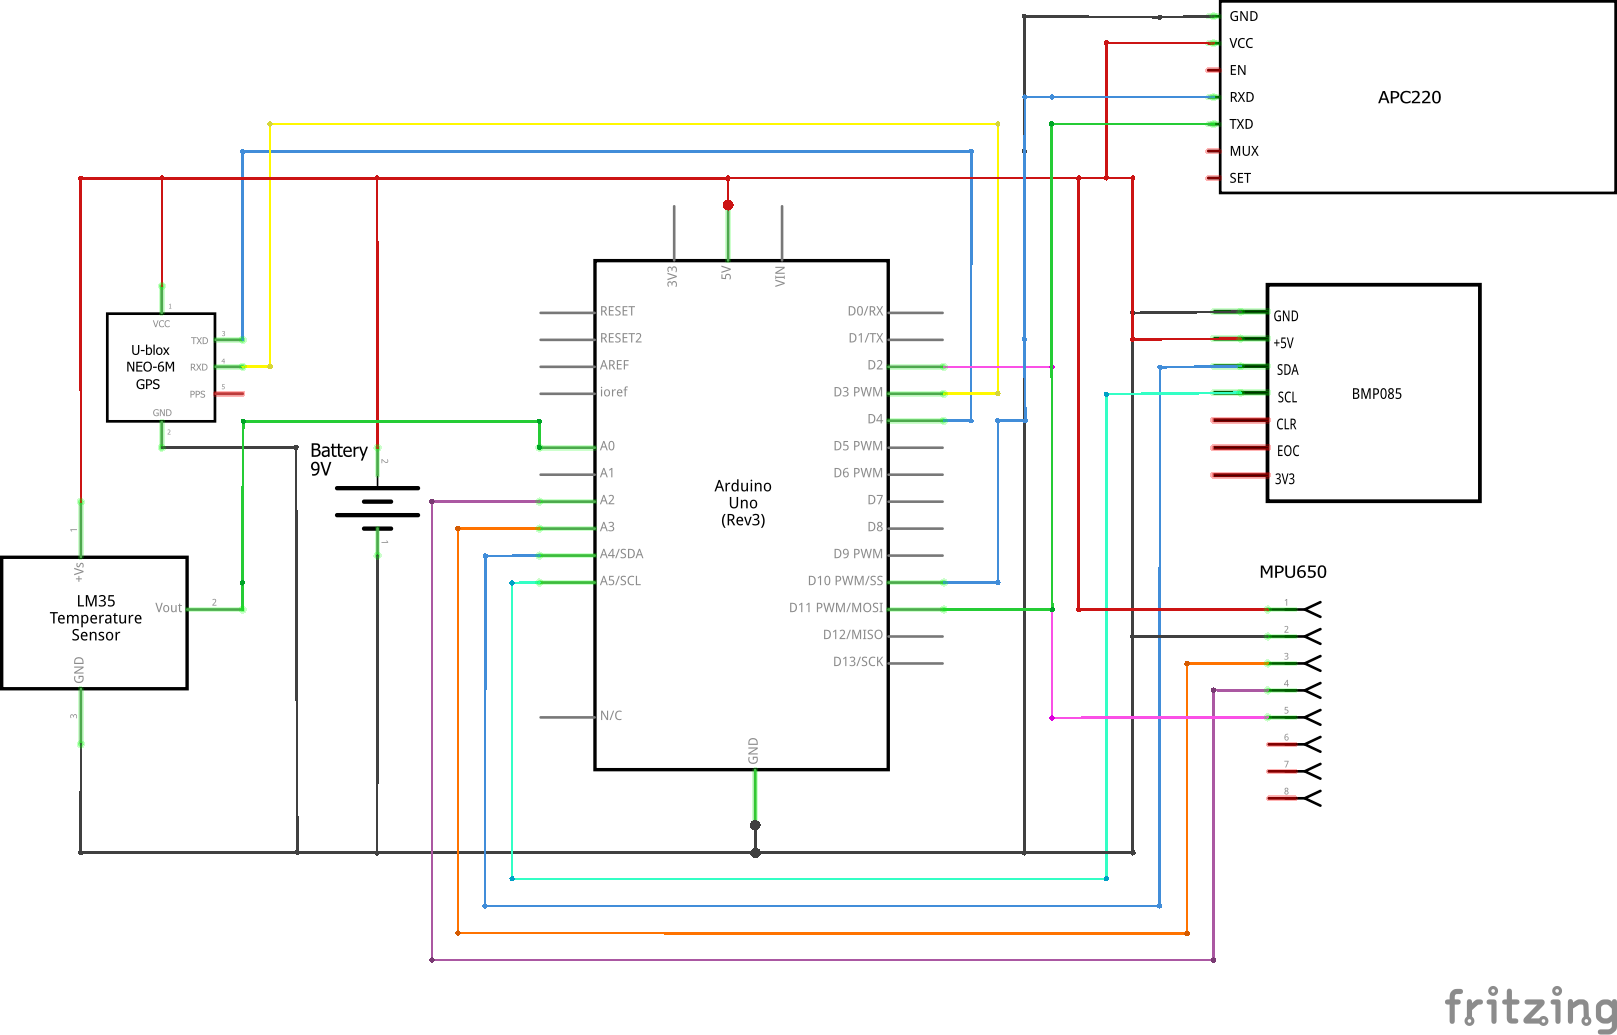
\includegraphics[width=0.9\linewidth]{electric_scheme}
\caption{Electronic circuit}
\end{figure}

\subsubsection{Radio Communication}

As we mentioned, we are using an APC220 for radio communication. This is for a couple of reasons, most importantly being its maximum transmission range: 1200 metres. We can also buy a second APC220 with a USB adaptor and connect it to our laptop, from the ground. We chose radio as our transmission method over wifi (via an ESP32), which has an inferior range of 200 metres. Internet transmission had the advantage of allowing us to use a more powerful protocol such as MQTT, a standard in IoT messaging. With our actual radio transmission, the CanSat computer sends a continuous stream of binary data, coupled with an error detection algorithm (Cyclic Redundancy Check), to ensure data integrity.

\subsubsection{Power Consumption}

The power budget for the CanSat is as follows:

\begin{table}[H]
\centering
\begin{tabularx}{\textwidth}{|X|X|}
\hline
Component           & Power Consumption \\ \hline
Arduino UNO R3      & 1.5 W             \\
APC220              & 0.75 W            \\
MPU6050             & 0.004 W           \\
NEO-6M              & 0.07 W            \\
LM35DZ              & 0.000006 W        \\
BMP085              & 0.000005 W         \\ \hline
Total               & $ \sim $ 2.5 W     \\ \hline
\end{tabularx}
\end{table}

A 9V battery can provide about 4.5 W hours of power, which means our payload can be powered on for about one hour and a half.

\subsection{Software design}

We are using C++17 as a programming language. The CanSat's software is highly object-oriented, as most components are abstracted. This allows us to define virtual interfaces for the hardware, which can be implemented for the real components but also for mock hardware, to enable testing on a computer. As a coding standard, we are using the JSF AV. The tasks are executed within a super loop.

\subsubsection{Software program flow}

The program flow can be seen in the following diagram:

\begin{figure}[H]
\centering
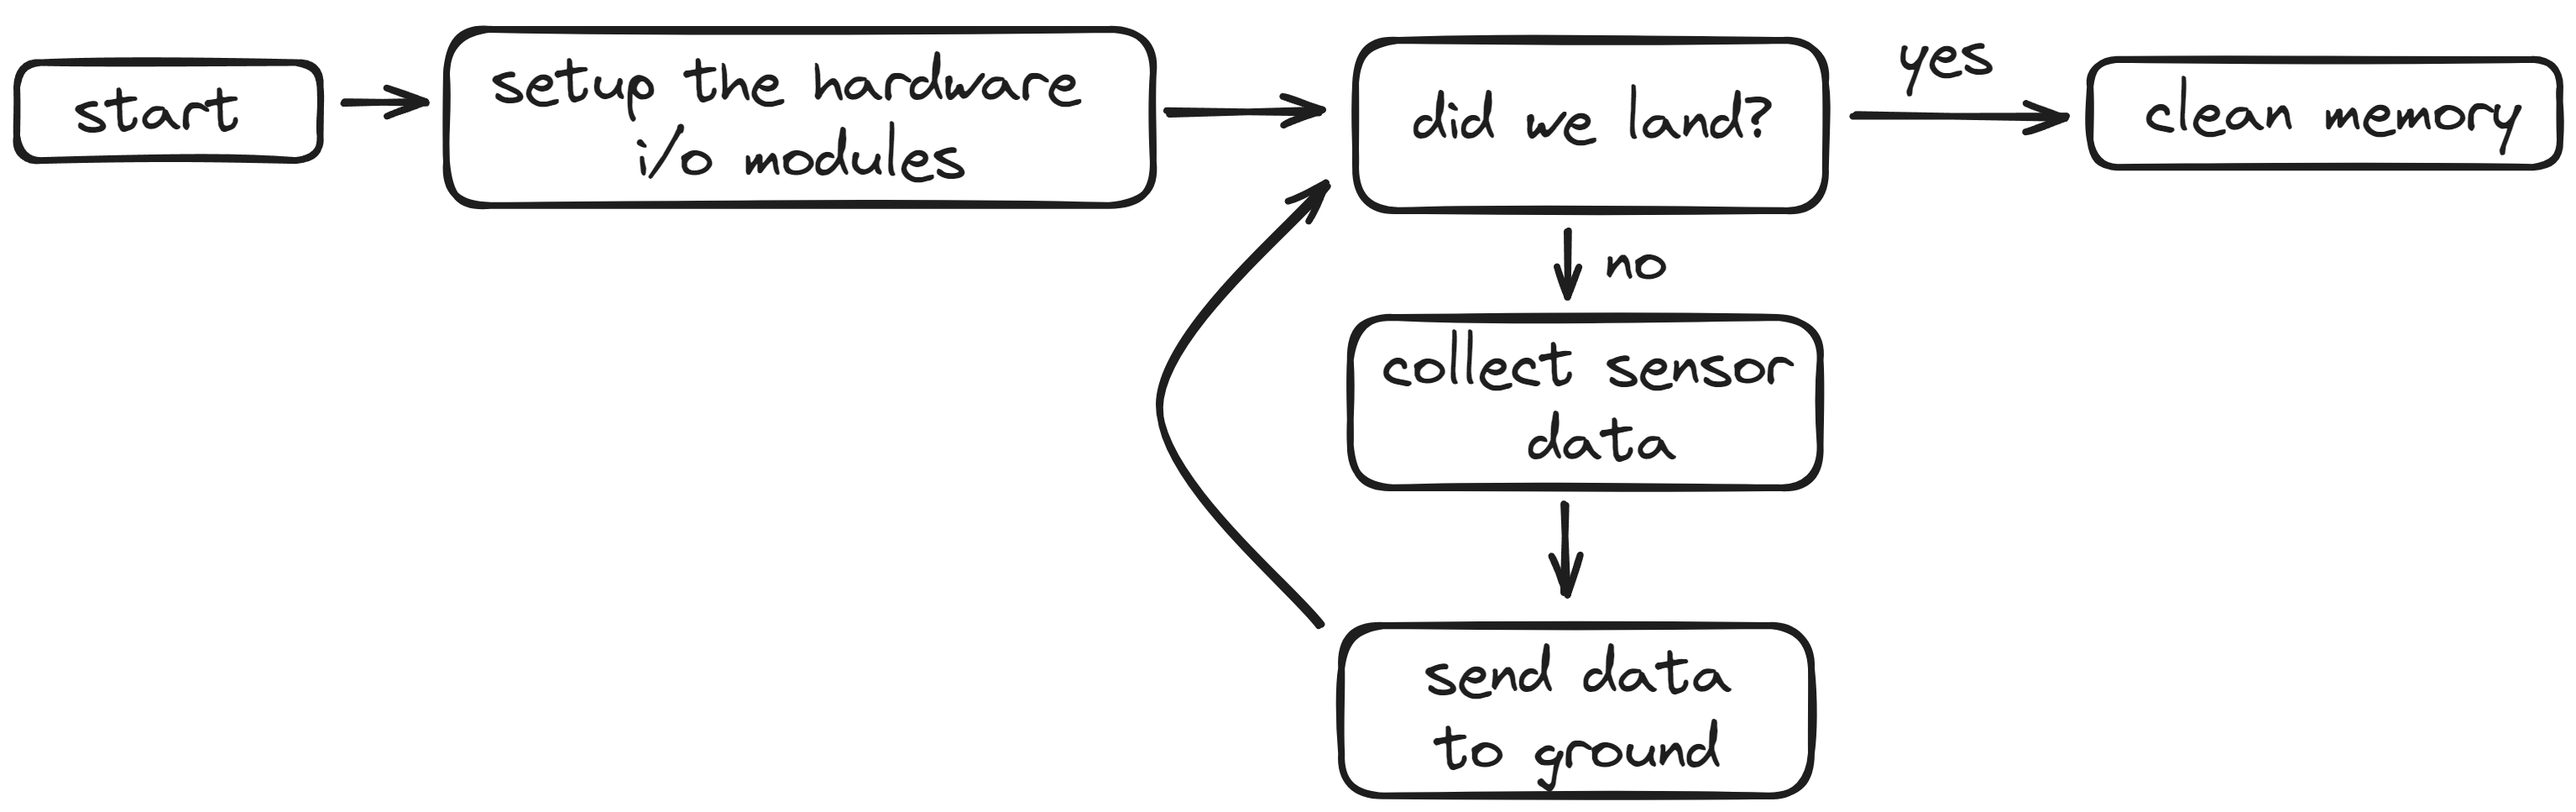
\includegraphics[width=0.9\linewidth]{flow_diagram}
\caption{Program flow}
\end{figure}

\subsubsection{Data Gathering and Storage}

To reduce complexity and costs, the CanSat doesn't store any long-term data. Instead, everything is transmitted to the ground station, where it's being processed and stored. The data is collected from the sensors, and sent via radio in a stream of binary data. We are using the Cyclic redundancy check (CRC) algorithm for error detection.To correct errors, the receiver (the ground station) has to send back an acknowledgement (ACK) or a negative acknowledgement (NACK). This process might add complexity, by requiring communication between the two devices. However an algorithm such as Forward error correction, which basically sends duplicate packets to correct any errors, adds too much garbage data and we need data fast to account for the entire duration of the mission, we can't afford any lag in our live data stream.

\subsubsection{Development Environment}

We are using an Arduino UNO as a microcontroller, which is powered by an ATmega328P microchip. To develop for this hardware, we are using the AVR toolchain. The code is written in C++17 and compiled with the avr-g++ compiler, and it's uploaded to the microcontroller using the avrdude command line tool. As a build tool, we are using GNU Make (makefiles).

\subsection{Recovery system}

Our rocket model will use a parachute with the diameter 417 mm for the recovery of the body tube and one with the diameter 217 mm for the recovery of the payload. For an optimum landing, we have chosen a cluster of two Aerotech D9-5 motors, both with a delay of 5 seconds. As it runs out of fuel, the rocket reaches its apogee, and, after the 5 second delay, the loose black powder in the motors will build pressure inside the body tube, pushing the nose cone out, since the shoulder will intentionally not be very tight, to allow the safe deployment of our payload and the two parachutes. Additionally, since we are using a cluster mount, we are reducing the risk of our motors failing to fire the ejection charge.

After subsequent tests, we will determine whether the pressure is too high and we need to add vents, small holes in the body tube, in order to let some of the pressure out and avoid a strong explosion, which would damage the payload.

Alternatively, if this method is deemed to be unsafe, too risky, or not efficient enough, we can deploy the payload and parachutes electronically, after our sensors indicate that apogee has been reached. [6]

\subsection{Ground support equipment}

The group equipment for the CanSat mission is composed of a laptop, with an APC220 radio receiver connected to it via a USB-C adaptor. The antenna is used to transmit and receive the data signals. The ground device has to respond with an acknowledgment (ACK) packet if the CRC checksum matches, so the CanSat knows there aren’t any errors in the transmitted data and can move on sending more packets. Otherwise, if the checksum doesn’t match, the receiver will reply with a negative acknowledgement (NACK) and the CanSat will send that packet again, hopefully without the same errors. More about the ground support device in the data analysis chapter. 
